
%============== N E W  ==== C H A P T E R  ======== 
\newpage
\chapter{Anhang} 
\index{Souce-Code|(}
\label{sec:Anhang} 

%============== N E W  ==== S E C T I O N  ======== 
\section{Screenshots zum Server}
\label{sec:Screenshots}

%============== N E W  ==== S U B - S E C T I O N  ======== 
\subsection{Shared Memory vor dem Einf�gen eines neuen Files}

\begin{figure}[h!]
\centering
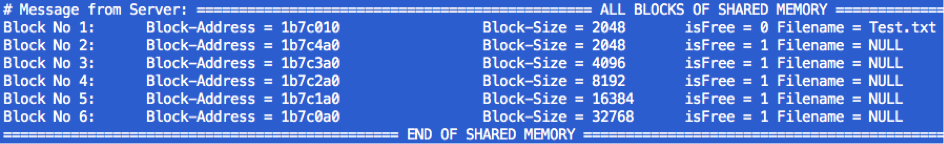
\includegraphics[width=1\textwidth]{screenshot-shm-1.png} 
\caption[SHM vor dem Einf�gen eines neuen Files]{SHM vor dem Einf�gen eines neuen Files\\Quelle: eigener Screenshot}
\label{fig:shm-1}
\end{figure}

%============== N E W  ==== S U B - S E C T I O N  ======== 
\newpage
\subsection{Aufteilen des Shared Memory in der Funktion devide()}

\begin{figure}[h!]
\centering
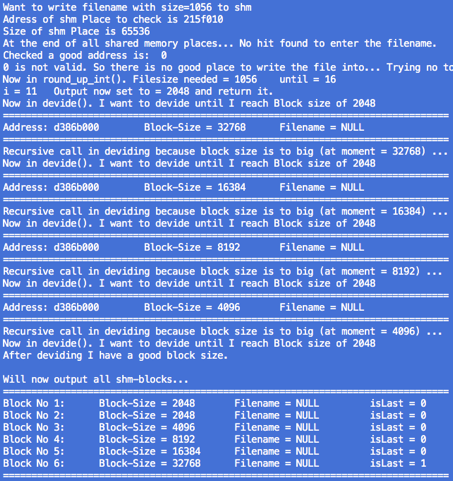
\includegraphics[width=1\textwidth]{screenshot-shm-2.png} 
\caption[Aufteilen des SHM in der Funktion devide()]{Aufteilen des SHM in der Funktion devide()\\Quelle: eigener Screenshot}
\label{fig:shm-2}
\end{figure}

%============== N E W  ==== S U B - S E C T I O N  ======== 
\newpage
\subsection{Shared Memory nach dem Einf�gen eines neuen Files}

\begin{figure}[h!]
\centering
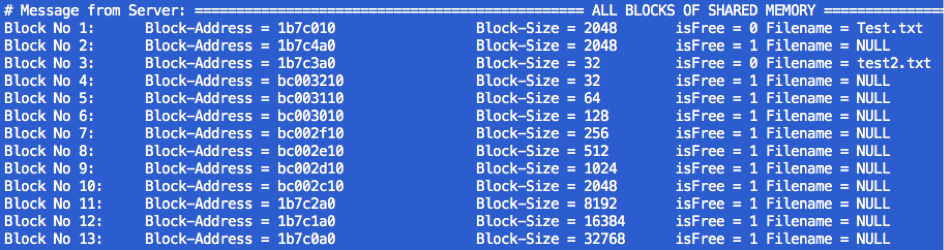
\includegraphics[width=1\textwidth]{screenshot-shm-3.png} 
\caption[SHM nach dem Einf�gen eines neuen Files]{SHM nach dem Einf�gen eines neuen Files\\Quelle: eigener Screenshot}
\label{fig:shm-3}
\end{figure}

%============== N E W  ==== S E C T I O N  ======== 
\newpage
\section{Programm-Code}
\label{sec:Program-Code}
%============== N E W  ==== S U B - S E C T I O N  ======== 
\newpage
\subsection{Aufteilen des Shared Memory in der Funktion devide()}
\lstset{language=c, mathescape=true}
\lstinputlisting[label=listing:devide,captionpos=b, caption=devide() - Aufteilen der Bl�cke des SHM]{dir/Anhang/listings/devide.c}



%============== N E W  ==== S U B - S E C T I O N  ======== 
\subsection{CREATE}
\label{Asubsec:CREATE}
\lstset{language=c, mathescape=true}
\lstinputlisting[label=listing:CREATE,captionpos=b, caption=CREATE - Funktionsweise]{dir/Anhang/listings/CREATE.c}


%============== N E W  ==== S U B - S E C T I O N  ======== 
\newpage
\subsection{READ}
\label{Asubsec:READ}
\lstset{language=c, mathescape=true}
\lstinputlisting[label=listing:READ,captionpos=b, caption=READ - Funktionsweise]{dir/Anhang/listings/READ.c}


%============== N E W  ==== S U B - S E C T I O N  ======== 
\newpage
\subsection{UPDATE}
\label{Asubsec:UPDATE}
\lstset{language=c, mathescape=true}
\lstinputlisting[label=listing:UPDATE,captionpos=b, caption=UPDATE - Funktionsweise]{dir/Anhang/listings/UPDATE.c}


%============== N E W  ==== S U B - S E C T I O N  ======== 
\newpage
\subsection{DELETE}
\label{Asubsec:DELETE}
\lstset{language=c, mathescape=true}
\lstinputlisting[label=listing:DELETE,captionpos=b, caption=DELETE - Funktionsweise]{dir/Anhang/listings/DELETE.c}

